\documentclass[letter,11pt,oneside]{article}
%%% HEREHEREHERE
%%% APPENDIX
%%% (insert (format "\n%s\n" (buffer-file-name)))
%%% /home/git/external/WRStars/documents/WRStars.tex

%%% (occur "\\(\\\\[a-z]*section\\|appendix\\|input\\|\\<include\\>\\)")
% /home/git/external/WRStars/documents/WRStars.tex
%%\documentclass[11pt,twocolumn]{article}
%%\usepackage[inline]{asymptote}       %% Inline asymptote diagrams
%%\usepackage{wglatex}                 %% Use this one and kill others.
\usepackage{color}                     %% colored letters {\color{red}{{text}}
\usepackage{fancyhdr}                  %% headers/footers
\usepackage{datetime}                  %% pick up tex date time 
\usepackage{lastpage}                  %% support page of ...lastpage
\usepackage{times}                     %% native times roman fonts
\usepackage{textcomp}                  %% trademark
\usepackage{amssymb,amsmath}           %% greek alphabet
\usepackage{parskip}                   %% blank lines between paragraphs, no indent
\usepackage{shortvrb}                  %% short verb use for tables
\usepackage{lscape}                    %% landscape for tables.
\usepackage{longtable}                 %% permit tables to span pages wg-longtable
\usepackage{multicol}                  %% Enhance footnotes/endnotes
\usepackage{url}                       %% Make URLs uniform and links in PDFs
\usepackage{enumerate}                 %% Allow letters/decorations for enumerations
\usepackage{endnotes}                  %% Enhance footnotes/endnotes
\usepackage{listings}                  %% Make URLs uniform and links in PDFs
\usepackage{rotating}                  %% sidewaysfigure
\pdfadjustspacing=1                    %% force LaTeX-like character spacing
\usepackage{geometry}                  %% allow margins to be relaxed
%%\usepackage{wrapfig}                 %% permit wrapping figures.
%%\usepackage{subfigure}               %% images side by side.
\geometry{margin=1in}                  %% Allow narrower margins etc.
\usepackage[T1]{fontenc}               %% Better Verbatim Font.
\renewcommand*\ttdefault{txtt}        %% 
\usepackage[colorlinks=true]{hyperref} %% Make huperlinks within a PDF
\usepackage{natbib}                    %% bibitems
\usepackage{upquote}                   %% make programmer's quoetes in verbatim sections.

%% include background image (wg-document-page-background) 

\usepackage{graphicx}            %% Include pictures into a document
%% (wg-texdoc-inserttikz)


\def\documentisdraft{DRAFT}

%% (wg-texdoc-isdraft)


\def\drafttest{DRAFT}
\def\wgdocdate{13 May, 2026}
\def\wgdocdatetime{\wgdocdate at \currenttime}
\ifx\documentisdraft\drafttest
\usepackage[left]{lineno}   %%%%%%%%%%%%% DRAFT
\usepackage{draftwatermark}
%%\SetWatermarkScale{5.0}
\SetWatermarkColor[gray]{0.9}
\fi

%% (wg-texdoc-insert-fancy-headers)

%%\usepackage[bookmarks]{hyperref} %% Make huperlinks within a PDF
%%\usepackage{makeidx}             %% Make an index uncomment following line
%%\makeindex                       %%.. yeah this one, too. index{key} in text
%%



\definecolor{verbcolor}{rgb}{0.6,0,0}
\definecolor{darkgreen}{rgb}{0,0.4,0}
\newcommand\debate[1]{\textcolor{darkgreen}{DEBATE: #1} \marginpar{\textcolor{red}{DEBATE} }}
\newcommand{\ltodo}[2]{\marginpar{\textcolor{red}{ACTION: #1}\endnote{#2}}}
\renewcommand{\thefigure}{\thesection-\arabic{figure}}
\newcommand{\menu}{\ensuremath{\;\rightarrow\;}}
\newcommand{\dhl}[1]{{\color{verbcolor}{\texttt#1}}}
\definecolor{wglightgreen}{rgb}{0.88, 0.58, 0.88}
\newcommand{\wgtextbox}[1]{\noindent\fcolorbox{darkgreen}{wglightgreen}{%
    \minipage[t]{\dimexpr0.80\linewidth-2\fboxsep-2\fboxrule\relax}
        {#1}
    \endminipage}}

%%(wg-latex-snippet)

%%(wg-add-inline-images)  %% add inline images to the mix




%%Begin User Definitions: Hint: ~/.latex.defs and  latex.defs  
%%End User Definitions:

%% (wg-texdoc-adjust-paper-width)
%% (wg-texdoc-insert-hypersetup)

%%% PDF Fields uncomment \usepackage[bookmarks]{hyperref} above.
\hypersetup{
colorlinks=true,
linkcolor=red,
citecolor=blue,
urlcolor=blue,
pdfauthor = {Copyright(c) 2020. All rights reserved. Wayne Green},
pdftitle = {Line Monitoring of elected Wolf-Rayet Southern Hemisphere Star Monitoring Campaign},
pdfsubject = {WR Preleminary Results, WR Stars},
pdfkeywords = {WR Stars, Spectroscopy},
pdfcreator = {LaTeX with hyperref package},
pdfproducer = {dvips + ps2pdf}}

%% (wg-latex-tablet-page)


%%%%%%%%%%%%%%%%%%%%%%%%%%%%%%%%%%%%%%%%%%%%%%%%%%%%%%%%%%%%%%%%%%%%%%%%%%%%%


\begin{document}


%% (wg-latex-pretty-title-page)
%% (wg-texdoc-titleblock)


\title{Line Monitoring of Selected Wolf-Rayet Southern Hemisphere Star Monitoring Campaign}
\author{Wayne Green$^{1}$, Anthony Rodda$^{2}$, John Wetmore$^{3}$\\
{\small $^{1}$\url{dxwayne@gmail.com},  $^{2}$\url{roddatony@gmail.com}, $^{3}$\url{john@azdesertskies.com} }}
\date{\today}
\maketitle

\begin{abstract}

We conducted a campaign of low resolution (R~1800) spectrographic
observations of a selected list of brighter southern hemisphere
Wolf-Rayet and O(f) stars using the FlexSpec1/600 and FlexSpec1/900
spectrographs with the Watson 24-inch CDK telescope located at the
Obstech observatory complex in Chile. This paper reports some
preliminary results from the on-going campaign. In this paper we
discuss the observational procedure, some of the issues encountered,
reduction approaches and techniques. The authors are grateful for the
generous allotment of time with Dr. Stan Watson's telescope
facilities.

\end{abstract}

%%%%%%%%%%%%%%%%%%%%%%%%%%%%%%%%%%%%%%%%%%%%%%%%%%%%%%%%%%%%%%%%%%%%%%%%%%%%%
%% table of contents
%%%%%%%%%%%%%%%%%%%%%%%%%%%%%%%%%%%%%%%%%%%%%%%%%%%%%%%%%%%%%%%%%%%%%%%%%%%%%
 
\pagenumbering{roman}   % i,ii,etc
%%\pagenumbering{gobble}   %ignore page numbers for a while
\pdfbookmark[0]{Table of Contents}{MyTOC} % if usepackage{hyperref} in use.
%%\tableofcontents
%%\listoffigures
%%\listoftables
%%\newpage


\setcounter{section}{0}
\pagenumbering{arabic}

\ifx\documentisdraft\drafttest
\linenumbers    %%%%%%%%%%%%% DRAFT
\fi

\section{Overview}

A campaign of observing bright Wolf-Rayet stars, magnitudes < 11.0
and declinations < -5 degrees was conducted using the custom FlexSpec1
R\textasciitilde 1100 spectrograph mounted to a Planewave CDK-24 on
an L600 mount located at Obstech Observatory, Chile. Early in the
project we added a R\textasciitilde 150 spectrgraph in anticipation
of observing fainter targets. Both instruments use a QHY 268M camera.

We share the telescope with top amateur LGRB imagers, and made our
observations during the bright-time, 10-day interval around full moon.
We start with targets in the west, work backwards towards the meridian,
and spend the most time on the meridian. We observed our target stars on
every clear night - airmass permitting.

% \ltodo{A0V paper}{Get title and bib ref}

As part of this campaign, we used available A0V stars as references. The
reference stars are covered in the accompanying paper. 

Targets were selected using a SIMBAD query for WR stars, conditioned
and saved in a comma-separated-file. This file was loaded into TOPCAT,
extended with the SIMBAD cross-match tool. Complete information for
targets was written to a PostgreSQL database. A similar technique
compiled the AOV stars. A subset of candidates based on magnitude,
field contamination, accessibility to Obstech, Chile was created
for use at the telescope. All coordinates are in decimal degrees,
but carrying the sexigesimal format allowed interface to the Planewave
'Favorites' list. Recently we learned the python interface to
Planewave scopes uses decimal degrees. 

\section{Observations}

During observations, the two tables were sent to Aladin using the
TOPCAT interop functionality sending sky coordinates and row
indices. The ra/dec were cross tied to the tables such that selecting
a star in the table would position Aladin to the field and
vice-versa. In Aladin, target stars were denoted with large, solid red
circles where reference stars were indicated with large, solid blue
circles. The reference stars were chosen by zooming out in Aladin
where the DSS color image was the default image used. This provided a
subject guess to extinction for the WR stars and helped to avoid the
inevitable crowded fields. Additional overlays of dim Gaia stars help
reject candidates with possible slit contamination. The star pairs
were recorded in one table together with the exposure time sequences.

The main computer for the telescope is a Windows 11 based environment
to meet ASCOM \cite{ASCOM2026} requirements for the equipment. Remote
operations were done in real-time using the RVNC viewer. We later
switched to TightVNC and Tailscale A JetKVM switch was added to the
Chile machine allowing for a web-based interface to the main machine
at the bios level. This permits un-wedging the machine during update
scenarios that require human intervention before the VNC servers start.

Two shared folders were created allowing access of files accumulating
in Chile by observers in Chile, Colorado and Arizona in the USA, and
Newcastle Upon Type in England. This brings Linux based analysis tools
to bear for quick checks of the data. We used SAOImage ds9
\cite{2003ASPC..295..489J} to examine images via the VNC link. This
saved us early on, as the magnitudes of some emission features
saturated, where the continuum was well within limits. In these cases
we took short exposures to fix the flux of bright features and longer
exposures to bring out lesser line details.

Recently we changed the R1100 spectrograph, to use a 1800 lmm grating
giving a R3200. 

\section{Results}

Preliminary reductions were performed with the Demetra \cite{demetra2026} software
package, images below are from PlotSpectra \cite{PlotSpectra}. The packaged handled image
acquisition and initial trimming using their crop image feature. Images
are not binned. Early in the campaign we noticed we were saturating
the large emission features, an event that was not well reported in
Demetra. This was determined with the 'Pixel Analysis' table in
SAOImage/DS9.  For some targets short exposures were used to fully
capture the emission features at the expense of smaller significant
lines, followed by longer exposures to gain sufficient SNR in the
smaller features.

Later processing followed the usual zero (bias) subtraction,
extraction of the apertures one at a time and individually wavelength
calibrated. The features were subjected to the IRAF \cite{2006hstc.conf..437G} clean step, and we
found boxcar windowing by 3 or three steps helped to clean the images,
at the expense of resolution. We are conducting a more precise
examination of images now, using continuum subtraction and
flux calibration.

We found PHD2 Guider \cite{phd2guider} to be offer high repeatability in placing the
target stars on the slit using their 'set and restore'
function.

Observations reveal a wide, non-periodic and quasi-periodic 
variation in spectral features. Quasi-periodic results are
from reported doubles where the period of variation covers
periods of approximately one year.


\section{Conclusions}

These are preliminary results, presented here to promote the idea
that WR and similar emission targets could be handled by use
of narrow passband (10nm) filters for continuous monitoring
at a much faster cadence, more targets per night, smaller
apertures etc. When important changes are detected, we then
bring the larger apertures to bear.

\section{Acknowledgments}

We appreciate the support from Dr. Stanley Watson for the 10 days of bright time observations
over these past two years. Special thanks to Anthony Rodda for travel, installation
and upgrades to the telescope. We extend special thanks to Ken Williams for his help
with the remote communications and general IT support of the computer environment.



\appendix
\renewcommand \thesection{\Alph{section}}


\begin{table}[h!]
{\small
\centering
\begin{tabular}{| l | l | l | l | l | l | l | l | l | l | l | l |}
\hline
  main\_id  & sp\_type &   ra\_d    &   dec\_d   &   u     &   b     &   v     &   r     & i  &   j    &   h    &   k       \\ 
\hline
 HD  62910  & WN6/WC4  & 116.24259  & -31.90821  & 10.080  & 10.440  & 10.100  & 10.170  &    & 8.570  & 8.322  & 7.928    \\ 
 HD  63099  & WC4+O7   & 116.46000  & -34.33014  & 11.470  & 11.430  & 10.500  & 10.370  &    & 8.452  & 8.110  & 7.545    \\ 
 HD  76536  & WC       & 133.74653  & -47.59241  &  9.040  &  9.130  &  8.800  &  9.520  &    & 7.486  & 7.245  & 6.612    \\ 
 HD 115473  & WC5      & 199.61664  & -58.13711  &  9.090  &  9.680  &  9.000  &  9.720  &    & 8.411  & 8.206  & 7.555    \\ 
\hline
\end{tabular}
\caption[TOC]{Characteristics of the sample results.}
\label{table:Characteristicsofthesampleresults.}
}
\end{table}


\begin{figure}[h!]
\centering
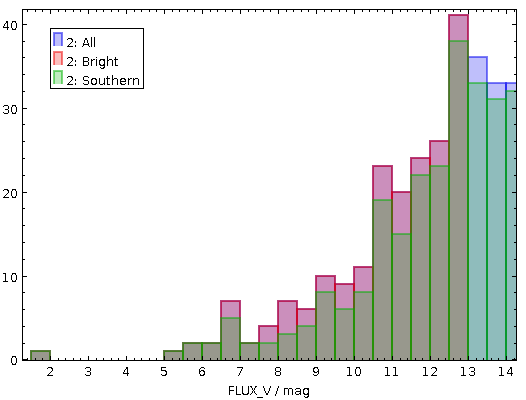
\includegraphics[width=\textwidth]{images/WRHistogram.png}
\caption{Histogram of WR stars in catalog.} %% \caption{{\tiny{citation}}} 
\label{figure:histogram}
\end{figure}

\clearpage

%%\begin{landscape}
\begin{figure}[h!]
\centering
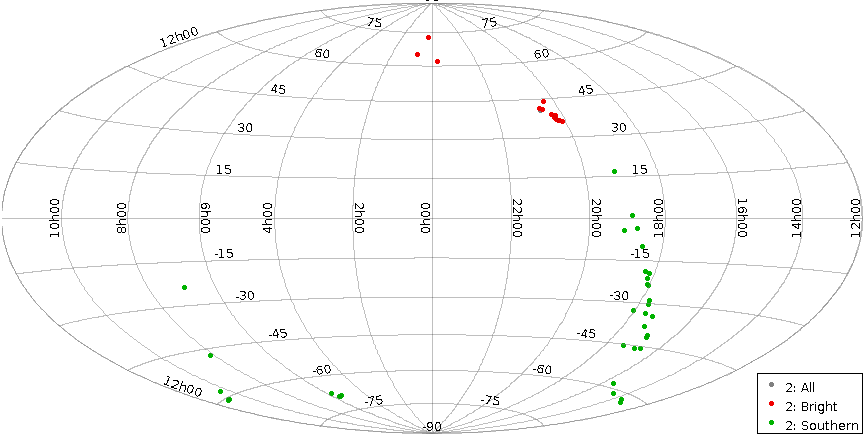
\includegraphics[width=\textwidth]{images/WRAtoff.png}
\caption{Sky location of 1,695 star.} %% \caption{{\tiny{citation}}} 
\label{figure:atoff-diagram}
\end{figure}
%%\end{landscape}



\section{Preliminary Results}

Observations range from 15 August, 2024 through 18 Feb, 2025 in
these preliminary results.



\begin{figure}[h!]
\centering
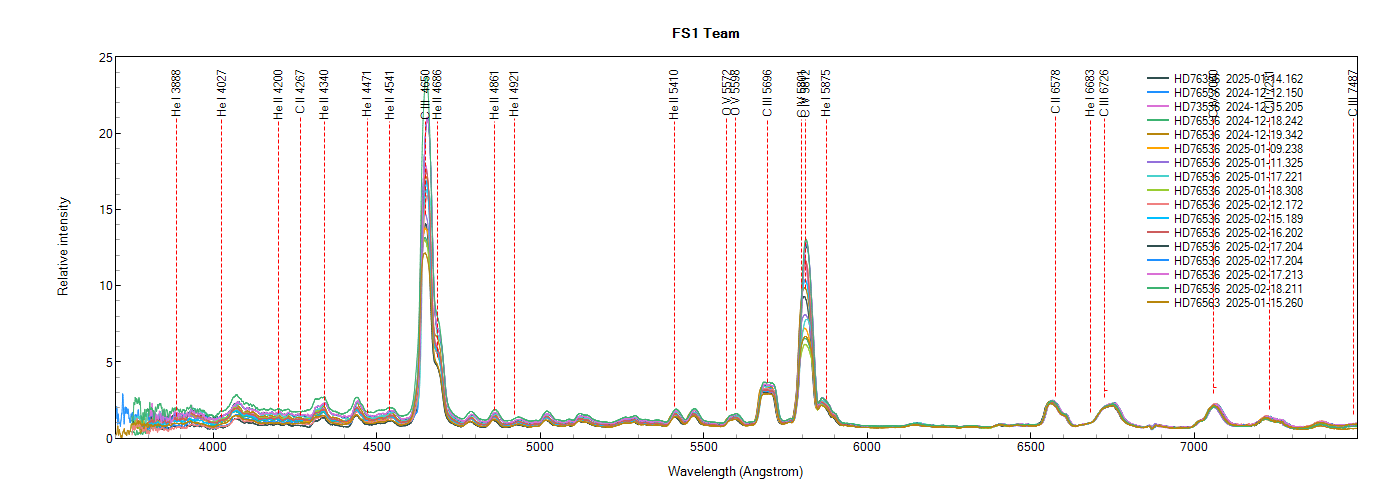
\includegraphics[width=\textwidth]{images/HD76536-FS1-Team.png}
\caption{HD76536  \tiny{FS1 Team}}
\label{figure:HD76536}
\end{figure}

\begin{figure}[h!]
\centering
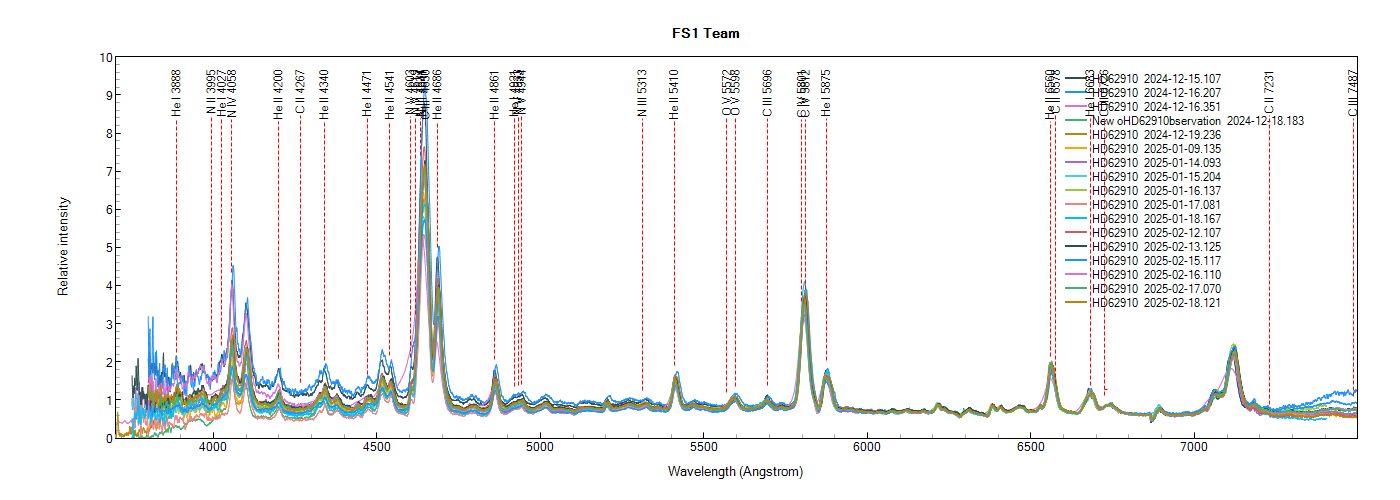
\includegraphics[width=\textwidth]{images/HD62910-FS1-Team.png}
\caption{HD62910 \tiny{FS1 Team}}
\label{figure:HD62910}
\end{figure}

\newpage
\begin{figure}[h!]
\centering
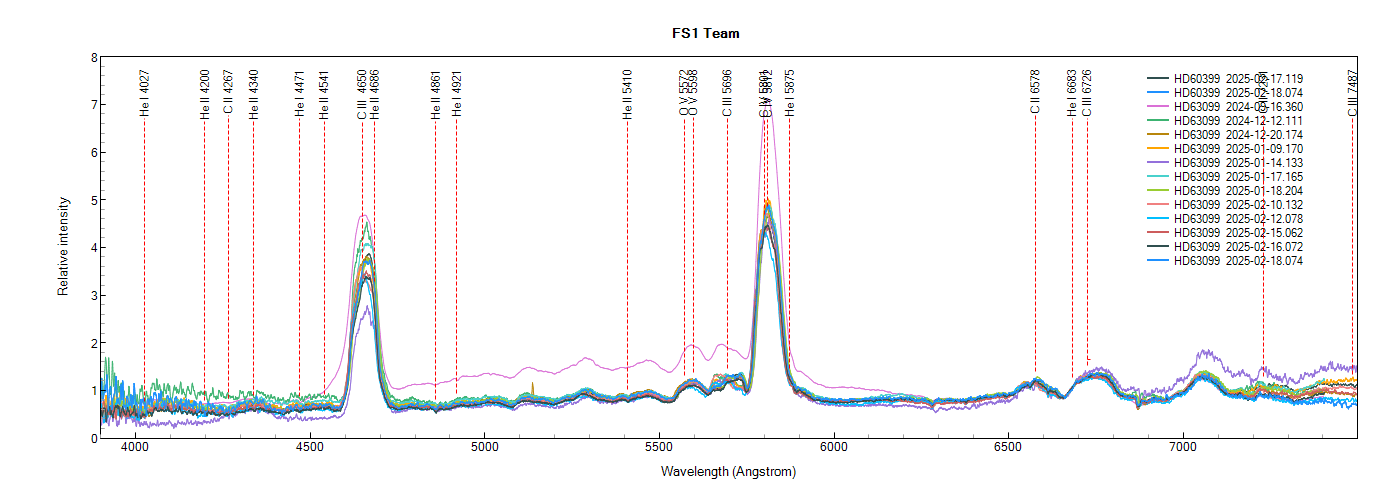
\includegraphics[width=\textwidth]{images/HD60399-FS1-Team.png}
\caption{HD60399 \tiny{FS1 Team}}
\label{figure:HD63099}
\end{figure}


\begin{figure}[h!]
\centering
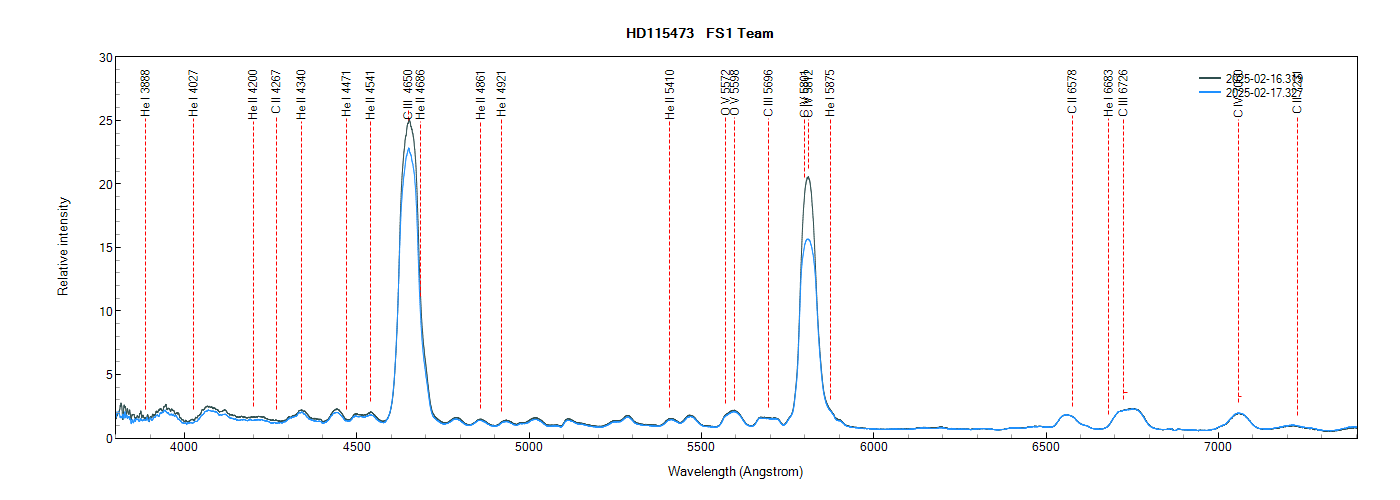
\includegraphics[width=\textwidth]{images/HD115473-FS1-Team.png}
\caption{HD115473 \tiny{FS1 Team}}
\label{figure:HD115473}
\end{figure}


%% use a bibitem approach to the references publications etc.
%% (wg-bibitem)

%%\clearpage
\addcontentsline{toc}{section}{References}
\renewcommand*{\refname}{My Bibliography and References}
\bibliographystyle{apalike}	% bibliographystyle{apalike} and \usepackage{natbib}
\bibliography{WRStars}	% expects file "MasterBib.bib"



%%\begin{thebibliography}{80}
%%\usepackage{natbib}   %% bibitems
%%\end{thebibliography}

%%\clearpage
%%\addcontentsline{toc}{section}{Index}
%%\printindex %% www.cs.usask.ca/resources/tutorials/latex/notes/toc-index.pdf

% /home/git/external/WRStars/documents/WRStars.tex

%% (wg-texdoc-endnotes)

%%%%%%%%%%%%%%%%%%%%%%%%%%%%%%%%%%%%%%%%%%%%%%%%%%%%%%%%%%%%%%%%%%%%%%%%%%%%%
% Support for endnotes
%% \begingroup
%% \renewcommand{\notesname}{\textcolor{red} {Action Items:}}
%% \parindent 0pt
%% \parskip 2ex
%% \phantomsection
%% \addcontentsline{toc}{section}{	extcolor{red} {Action Items:}}
%% \def\enotesize{\normalsize}
%% \theendnotes
%% \endgroup

\end{document}


select main_id, sp_type, ra_d::numeric(9,5), dec_d::numeric(9,5),
    u::numeric(7,3),
    b::numeric(7,3),
    v::numeric(7,3),
    r::numeric(7,3),
    i::numeric(7,3),
    j::numeric(7,3),
    h::numeric(7,3),
    k::numeric(7,3)
from wr_all_simbad
where main_id ~ '76536|62910|63099|115473'
order by ra_d;

  main_id  | sp_type |   ra_d    |   dec_d   |   u    |   b    |   v    |   r    | i |   j   |   h   |   k   
-----------+---------+-----------+-----------+--------+--------+--------+--------+---+-------+-------+-------
 HD  62910 | WN6/WC4 | 116.24259 | -31.90821 | 10.080 | 10.440 | 10.100 | 10.170 |   | 8.570 | 8.322 | 7.928
 HD  63099 | WC4+O7  | 116.46000 | -34.33014 | 11.470 | 11.430 | 10.500 | 10.370 |   | 8.452 | 8.110 | 7.545
 HD  76536 | WC      | 133.74653 | -47.59241 |  9.040 |  9.130 |  8.800 |  9.520 |   | 7.486 | 7.245 | 6.612
 HD 115473 | WC5     | 199.61664 | -58.13711 |  9.090 |  9.680 |  9.000 |  9.720 |   | 8.411 | 8.206 | 7.555




('HD76536','HD62910','HD62910','HD63099','HD115473')

where main_id_x ~ '76536|62910|62910|63099|115473'


select main_id_x, ra_d, dec_d from wrall 
where main_id_x ~ '76536|62910|62910|63099|115473'
order by ra_d;












%
We appreciate the support from Dr. Stanley Watson for the 10 days of bright time observations
over these past two years. Special thanks to Anthony Rodda for travel, installation
and upgrades to the telscope. We extend special thanks to Ken Williams for his help
with the remote communications and general IT support of the computer environment.
Start the project. Using table J/A+A/458/453/table1, the
Annex to 7th Cat. of Galactic WR Stars (van der Hucht, 2006).
with 119 stas. A SIMBAD search returned 1,695 stars.

WR Stars are bright > 8 M$_\odot$, with relativly short overall
life times. 

Most stars are well suited to summer/fall observations.
